\documentclass{report}

\usepackage{ptext}
\usepackage{lipsum}
\input{Boostan-UserManual}
\usepackage{graphicx}
\usepackage{tabularx}

\newword{Abstraction}{Abstraction}
{انتزاع}{}

\newword{Abstract}{Abstract}
{انتزاعی}{}

\newword{AbsoluteMinimum}{Absolute Minimum}
{کمینه مطلق}{}


\newword{AcceptableCell}{Acceptable Cell}
{سلول پذیرفتنی}{سلول‌های پذیرفتنی}

\newword{AccessBurst}{Access Burst}
{توده دسترسی}{توده‌های دسترسی}


%%% S
\newword{Sample}{Sample}
{نمونه}{نمونه‌ها}

\newword{SamplePath}{Sample Path}
{نمونه مسیر}{}

\newword{SampleSpace}{Sample Space}
{فضای نمونه}{فضای نمونه‌ها}
\newacronym{ACK}{ACK}{Acknowledgement}

\newacronym{ACI}{ACI}{Application Control Interface}

\newacronym{ACIR}{ACIR}{Adjacent Channel Interference Ratio}

\newacronym{ACLC}{ACLC}{Adaptive Configuration of Logical Channels}

\newacronym{ACLP}{ACLP}{Adjacent Channel Leakage Power}

\title{پروژه باریم
}
\type{
 درس آشنایی با شبکه های تلفن همراه }
\author{غزل عربعلی - 97521396، بهاره کاوسی نژاد - 99431217}
\logofile{Pic/IUST}


\begin{document}
\pagenumbering{gobble}
\maketitle
\pagenumbering{arabic}
\chapter{شرح پروژه}


گسترش روزافزون شبکه های تلفن همراه به ویژه شبکه های نسل چهار و پنج، موجب شده است که این شبکه ها به عنوان بزرگترین شبکه دسترسی
\footnote{\lr{Access Network}}
 ، برای دستیابی به خدمات اینترنت بشمار آید. پرواضح است که در این بین، مساله امنیت
 \footnote{\lr{Security}}
  برنامه های کاربردی
  \footnote{\lr{Application}}
  و ساخت یک برنامه کاربردی با یک ارتباط امن، یکی از مهم ترین مسایل این حوزه خواهد بود. گرچه باید به این نکته توجه داشت که امنیت در یک ارتباط از طریق شبکه های تلفن همراه را، نباید تنها به مساله امنیت در دو سوی مشتری
   \footnote{\lr{Client}}
   و خدمت گزار
   \footnote{\lr{Server}}
   تقلیل داد؛ بلکه در جای جای این ارتباط، ما می توانیم با حملات متعددی مواجه شویم، که می تواند محرمانگی
   \footnote{\lr{Confidentiality}}
   ، یکپارچگی
   \footnote{\lr{Integrity}}
    و حریم خصوصی
    \footnote{\lr{Privacy}}
     ما را هدف قرار دهد. شکل 
     \ref{fig:Client_Server}
      نمایی از ارتباط یک مشتری با خدمت گزار را در بستر های مختلف از طریق شبکه های تلفن همراه به زیبایی نشان می دهد.
  
   \begin{figure}[ht]
   	\centering
   	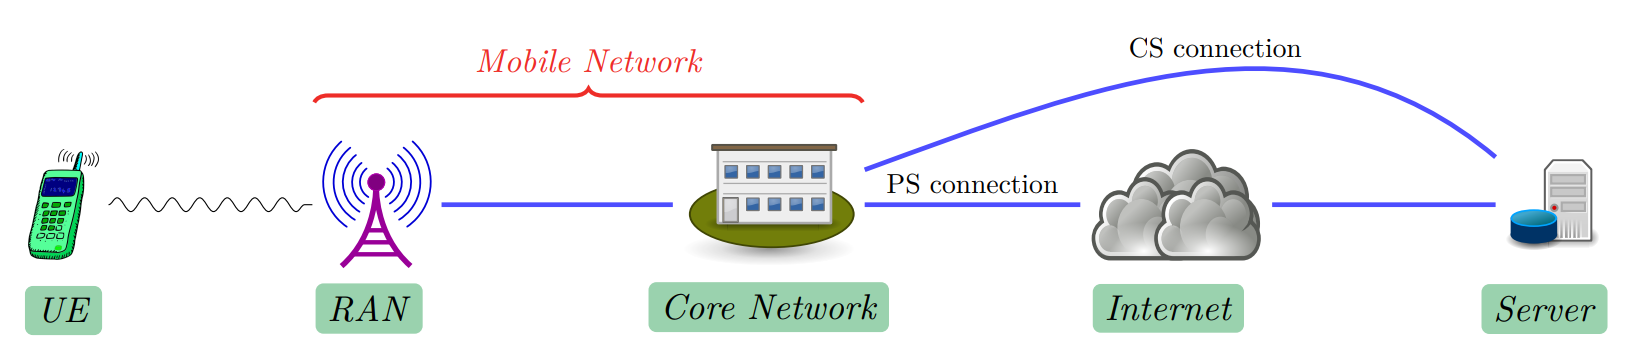
\includegraphics[width=\textwidth]{Pic/Client_Server}
   	\caption{ارتباط بین مشتری با خدمت گزار از طریق شبکه های تلفن همراه بر روی بسترهای مختلف}
   	\label{fig:Client_Server}
   \end{figure}
   
   در مساله پیش رو، فرض می کنیم که یک برنامه کاربردی داریم، که توسط برنامه 
   \lr{UE}
    می شود.
     \lr{UE}
      از دیدگاه ما هر ابزاری است که توسط آن بتوان به شبکه های تلفن همراه متصل شد.
       \lr{UE}
        می تواند گوشی تلفن همراه، تبلت و یا حتی هر شی در
         \lr{IoT}
         \footnote{\lr{Internet of Things}}
          باشد. گرچه در این پروژه، ما تنها بر روی گوشی های تلفن همراه و تبلت ها تمرکز خواهیم کرد.
          
   برنامه کاربردی
   \lr{UE}
    قرار است تا از طریق بسترهای موجود در شبکه های تلفن همراه به یک خدمت گزار مشخص متصل شوند و با آن تبادل اطلاعات داشته باشند. در این جا ما دو راه کار برای اتصال به خدمت گزار داریم. در راه کار نخست و بدیهی ترین شیوه، ما از طریق بستر اینترنت با خدمت گزار به تبادل داده مبادرت می ورزیم. ما اصطلاحا به این شیوه اتصال از طریق 
    \lr{PS}
    \footnote{\lr{Packet-switched}}
     می گوییم. بالاخره باید پذیرفت که دنیای اینترنت، مخاطرات پیدا و پنهان فراوانی دارد. اتصال از طریق خدمات
     \footnote{\lr{Service}} 
     \lr{CS}
     \footnote{\lr{Circuit-switched}}     
     نظیر تماس
     \footnote{\lr{Call}}
      و 
      \lr{SMS}
      \footnote{\lr{Short Message Service}}
     ، می تواند راه فراری از مخاطرات دنیای اینترنت باشد. در این پروژه، ما فرض می کنیم که اتصال مشتری به خدمت گزار را از طریق
      \lr{SMS}
      ، برقرار خواهد شد.
      
     \begin{figure}[ht]
     	\centering
     	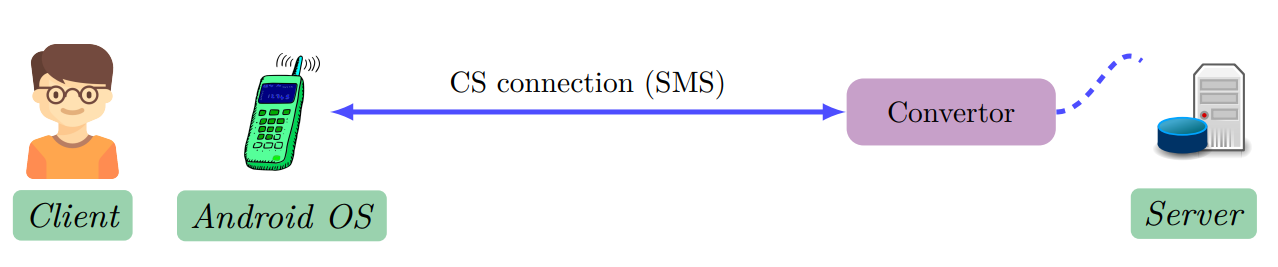
\includegraphics[width=\textwidth]{Pic/High_level_architecture}
     	\caption{معماری سطح بالای سامانه}
     	\label{fig:High_level_architecture}
     \end{figure} 

در این جا برای سادگی فرض کنید که دو گوشی داریم. گوشی سمت مشتری و گوشی که ما به عنوان خدمت گزار از آن استفاده می کنیم. در سمت خدمت گزار (که در حقیقت یک گوشی معمولی است)، یک برنامه
 \lr{Android}
 ای با کارکرد
  \lr{Backend} 
  نصب می شود.
مشتری از طریق
 \lr{SMS}
  فرمان ها را به سمت مقابل (خدمت گزار) ارسال می کند. مشتری می بایست به صورت مداوم اطلاعات مربوط به توان دریافتی و تکنولوژی سلول خدمتگزار
  \footnote{\lr{Serving Cell}}
  و مکان دریافت این اطلاعات را در صورتی که توان از یک سطح آستانه معین پایین بیاید در قالب یک پیام برای خدمت گزار ارسال کند. در این سامانه می بایست به نکات زیر دقت کنید:
  \begin{itemize}
  	\item
  	برنامه سمت خدمت گزار می بایست به صورت یک سرویس در 
  	\lr{Android} 
  	باشد، البته برای مدیریت و پیکربندی آن می توان یک برنامه
  	\lr{UI}
  	 دار نیز داشته باشیم.
  	\item
  	فرض کنید که همگان پروتکل ارتباطی شما را که مبتنی بر
  	 \lr{SMS}
  	  است می دانند. اگر اجازه دهیم
  	   \lr{SMS}
  	    از هر شماره ای به سمت خدمت گزار ارسال شود، رویه ای در نظر بگیرید که جلوی دسترسی های غیرمجاز را بگیرد. شاید یک رویه ساده، ارسال یک رمز عبور
  	    \footnote{\lr{Password}}
  	     در ابتدای
  	    \lr{SMS}
  	     است. تلاش کنید تا رویه های بهتری برای حل این چالش در نظر بگیرید.
  	\item
  	در هنگامی که مشتری درخواست خود را برای خدمت گزار ارسال می کند، خدمت گزار درخواست را می بایست اجرا کند و پاسخ را در یک
  	\lr{SMS}
  	 جداگانه برای مشتری ارسال کند. دقت کنید اگر بتوانید باید تشخیص بدهید که 
  	 \lr{Delivery}
  	 بر می گردد یا خیر. اگر برنگشت باید پیام را دوباره ارسال کنیم.
  	\item
  	در پیام ارسالی از سوی مشتری، می بایست مکان اندازه گیری، مقداری اندازه گیری و اطلاعات سلولی که به آن متصل است را ارسال کند.
  	\item 
  	پروتکل ارتباطی را باید به صورت کامل مستند بکنید، و باید مبتنی بر پروتکل 
  	\lr{SMPP}
  	\footnote{\lr{Short Message Peer-to-Peer}}
  	 باشد.
  \end{itemize}

\chapter{توضیحات کدها}
\section{فایل
\lr{SMPP.kt}
}
کلاس 
\lr{SMPP}
 که از
  \lr{DefaultSmppSessionHandler}
   به ارث برده شده، برای مدیریت جلسات
    \lr{SMPP}
     در یک برنامه
      \lr{Android}
       طراحی شده است. این کلاس شامل متغیرهایی برای نگهداری تنظیمات
        \lr{SMPP}
         (مانند میزبان، پورت، کاربر، و رمز عبور) و همچنین روشی برای پیکربندی این تنظیمات می‌باشد. متد
          \lr{configure}
           برای تنظیم جزئیات اتصال
            \lr{SMPP}
             استفاده می‌شود.

\subsection{متد
\lr{sendSMS}
}
متد
 \lr{sendSMS} 
 تلاش می‌کند تا یک پیام 
 \lr{SMS}
  به شماره داده شده ارسال کند. این متد ابتدا یک
   \lr{SMPP client} 
   و 
\lr{session} 
   ایجاد می‌کندو پیام را به قسمت‌هایی تقسیم می‌کند. با دو آستانه مقدار قدرت سیگنال را تست می کند. اگر سیگنال قدرت سلول سرویس‌دهنده کمتر از 
   \lr{-50}
   و یا
   \lr{-110}
    باشد، قسمت‌های پیام را ارسال می‌کند. سپس به مدت 
    10 
    ثانیه منتظر می‌ماند و در نهایت 
    \lr{session} 
    و 
    \lr{client} 
    را می‌بندد و از بین می‌برد. اگر خطایی رخ دهد، آن را در 
    \lr{log}
     ثبت می‌کند و مقدار 
     \lr{false} 
     را بازمی‌گرداند.

\subsection{متد
	\lr{getSessionConfig}
}
متد 
\lr{getSessionConfig} 
پیکربندی جلسه 
\lr{SMPP} 
را با استفاده از تنظیمات ذخیره شده در
 \lr{shared preferences} 
 بازمی‌گرداند. این متد یک شیء 
 \lr{SmppSessionConfiguration} 
 را ایجاد می‌کند و نوع جلسه، میزبان، پورت، شناسه سیستم، و رمز عبور را تنظیم می‌کند.
 
 \subsection{متد
 	\lr{createSubmitSm}
 }
متد
 \lr{createSubmitSm}
  یک شیء 
  \lr{SubmitSm} 
  ایجاد می‌کند که برای ارسال پیام
   \lr{SMS}
    استفاده می‌شود. این متد آدرس‌های مبدا و مقصد، کدینگ داده، و پیام کوتاه را تنظیم می‌کند و متن پیام را با استفاده از کاراکترست داده شده کدگذاری می‌کند.
\subsection{متد
	\lr{splitMessage}
}
متد
 \lr{splitMessage}
 پیام را به قسمت‌هایی با حداکثر طول بایت مشخص تقسیم می‌کند. این متد از یک کدکننده کاراکتر برای تبدیل پیام به یک
  \lr{buffer}
  بایت استفاده می‌کند و پیام را به قسمت‌هایی تقسیم می‌کند که هر کدام طولی کمتر از 
 \lr{maxByteLength} 
 دارند.
\subsection{متد
	\lr{extractServingCellSignalStrength}
}
متد 
\lr{extractServingCellSignalStrength} 
قدرت سیگنال سلول سرویس‌دهنده را از یک پیام استخراج می‌کند. این متد پیام را به بخش‌هایی بر اساس جداکننده ; تقسیم می‌کند و سپس اولین بخش را به عناصر جداگانه بر اساس , تقسیم می‌کند و قدرت سیگنال را به عنوان یک عدد صحیح بازمی‌گرداند.
\subsection{متد
	\lr{firePduRequestReceived}
}
در نهایت، متد 
\lr{firePduRequestReceived}
 که از
  \lr{DefaultSmppSessionHandler}
   به ارث برده شده، درخواست‌های
    \lr{PDU}
     دریافت شده را پردازش می‌کند. اگر کدینگ داده پیام 0 باشد، آدرس مبدا، مقصد، و محتوای پیام را چاپ می‌کند و یک پاسخ ایجاد می‌کند و بازمی‌گرداند.


\section{فایل
\lr{SMSActivation}
}
در کلاس 
\lr{SMSActivation}
 که از
  \lr{AppCompatActivity}
   به ارث برده شده، متغیرهای لازم برای مدیریت مجوزهای دسترسی به پیامک‌ها، آداپتور چت و آیتم‌های چت تعریف می‌شود. در متد
    \lr{onCreate}
    ، ابتدا چک می‌شود که آیا مجوز خواندن پیامک‌ها به برنامه داده شده است یا خیر. اگر مجوز داده نشده باشد، درخواست مجوز ارسال می‌شود و سپس پیامک‌ها خوانده می‌شوند. اگر مجوز قبلاً داده شده باشد، پیامک‌ها مستقیماً خوانده می‌شوند. سپس
     \lr{RecyclerView} 
     با استفاده از
      \lr{LinearLayoutManager} 
      مقداردهی اولیه می‌شود و آداپتور چت به آن متصل می‌شود. همچنین یک دکمه برگشت تنظیم می‌شود که با کلیک بر روی آن، فعالیت فعلی خاتمه می‌یابد.

\subsection{متد
\lr{updateChatItems}
}
در متد 
\lr{updateChatItems}
، آیتم‌های چت جدید جایگزین آیتم‌های فعلی می‌شوند و به آداپتور اطلاع داده می‌شود که داده‌ها تغییر کرده‌اند. این متد برای به‌روزرسانی آیتم‌های چت استفاده می‌شود. متد 
\lr{loadChatItems} 
نمونه‌ای از نحوه استفاده از این متد را نشان می‌دهد. در این متد، پیامک‌های جدید خوانده می‌شوند و سپس با استفاده از
 \lr{updateChatItems} 
 آیتم‌های جدید به‌روزرسانی می‌شوند.

\subsection{متد
	\lr{readSms}
}
متد 
\lr{readSms}
 پیامک‌های دستگاه را خوانده و آن‌ها را به لیستی از آیتم‌های چت تبدیل می‌کند. این متد ابتدا ستون‌های مورد نیاز برای خواندن پیامک‌ها (آدرس، متن و نوع پیامک) را مشخص می‌کند و سپس یک کوئری برای دریافت این داده‌ها از 
 \lr{contentResolver}
  ارسال می‌کند. در حالی که 
  \lr{cursor}
   به پیامک‌ها اشاره می‌کند، پیامک‌ها یکی یکی خوانده می‌شوند و اگر متن پیامک شامل عبارت 
   "
   \lr{SMPP}
   " 
   باشد، متن پیامک پاک‌سازی می‌شود و سپس به لیست آیتم‌های چت اضافه می‌شود. در نهایت 
   \lr{cursor}
    بسته می‌شود و لیست آیتم‌های چت بازگردانده می‌شود.
\subsection{متد
	\lr{SMSActivation}
}
در کلاس
 \lr{SMSActivation} 
 متغیرهای
  \lr{permission} 
  و 
  \lr{requestCode} 
  برای مدیریت مجوزهای دسترسی به پیامک‌ها استفاده می‌شوند. همچنین 
  \lr{recyclerView} 
  برای نمایش لیست پیامک‌ها،
   \lr{chatAdapter} 
   برای مدیریت آیتم‌های چت و 
   \lr{chatItems} 
   برای نگهداری لیست پیامک‌ها تعریف شده‌اند. این متغیرها در متد
    \lr{onCreate} 
    مقداردهی اولیه می‌شوند و تنظیمات اولیه برای نمایش پیامک‌ها و مدیریت تعاملات کاربر با دکمه برگشت انجام می‌شود.
    
    
\section{فایل
 \lr{SMSReceiver}
}  
کلاس
 \lr{SMSReceiver} 
 که از
  \lr{BroadcastReceiver} 
  به ارث برده شده است، برای مدیریت پیام‌های ورودی
   \lr{SMS} 
   طراحی شده است. در این کلاس، متد
    \lr{onReceive} 
    بازنویسی شده تا پیام‌های
     \lr{SMS} 
     ورودی را پردازش کند. وقتی یک پیام 
     \lr{SMS} 
     دریافت می‌شود، این متد فراخوانی می‌شود و پیام‌ها را از طریق
      \lr{intent} 
      دریافت می‌کند.

ابتدا، اگر
 \lr{bundle}
  که حاوی داده‌های پیام است، غیر 
  \lr{null}
   باشد، مجموعه‌ای از
    \lr{PDUs (Protocol Data Units)}
     از
      \lr{bundle} 
      استخراج می‌شوند. هر
       \lr{PDU} 
       به یک پیام 
       \lr{SMS} 
       تبدیل می‌شود و از آن شماره فرستنده و متن پیام استخراج می‌گردد. سپس این اطلاعات در
        \lr{log}
        برای اهداف اشکال‌زدایی ثبت می‌شود.

در مرحله بعد، چک می‌شود که آیا متن پیام حاوی عبارت "پیام شما دریافت شد" است یا خیر. اگر این عبارت در پیام یافت شود، یک
 \lr{intent}
 جدید برای شروع
  \lr{MainActivity} 
  ایجاد می‌شود. این
   \lr{intent} 
   شامل
    \lr{flag}
    هایی است که نحوه اجرای
     \lr{MainActivity} 
     را تعیین می‌کنند و اطلاعات مربوط به پیام را به صورت
      \lr{extras} 
      به آن اضافه می‌کنند.

در نهایت،
 \lr{MainActivity}
 با استفاده از 
 \lr{intent} 
 ایجاد شده و شامل اطلاعات پیام، آغاز می‌شود. این اقدام به 
 \lr{MainActivity} 
 اجازه می‌دهد که پیام را دریافت کرده و به آن پاسخ دهد یا آن را نمایش دهد. این فرآیند به طور کامل، امکان پردازش و مدیریت پیام‌های 
 \lr{SMS} 
 را در برنامه فراهم می‌آورد.
\chapter {مراجع}
\begin{itemize}
	\item 1
\end{itemize}
\end{document}
